\chapter{Úvod do problematiky}

\indent

V první kapitole bychom se měli seznámit s pojmem Ultimate Frisbee. Dále pak nastíníme
problematiku pořádání turnajů v tomto minoritním sportu.

\section{Co je to Ultimate Frisbee}

\indent

Ultimate Frisbee je mladý a dynamicky se rozvíjející sport s létajícím talířem,
který se hraje od roku 1968 \cite{cald-ultimate}. Hraje jej přibližně sedm miliónů
hráčů ve více než 80 zemích světa a jeho popularita rok od roku stoupá \cite{usa-ultimate}.
Během posledních několika let je například běžné sledovat živé přenosy na sportovním kanálu ESPN
z Amerických soutěží, především profesionální ligy AUDL. Ultimate v roce 2015 dokonce získalo
uznání od Mezinárodního olympijského výboru \cite{cald-uznani}. Nejčastěji se hraje v kategoriích
open (muži), ženy, mix (smíšené týmy mužů a žen), junioři (do 19 let) a masters (nad 33 let).

\subsection{Pravidla}

\indent

Popularitě přidává fakt, že jde o celkem vzato nenáročnou hru na vybavení s jednoduchými pravidly:

\begin{quote}
Ultimate je kolektivní bezkontaktní sport, v němž vítězí tým, který má na konci hrací doby
vyšší počet bodů. Hraje se na hřišti o rozměrech cca 100x37 metrů (délka fotbalového hřiště,
polovina jeho šířky). Na obou koncích hřiště jsou vyznačeny koncové zóny o hloubce cca 18 metrů.

V ultimate proti sobě hrají dva sedmičlenné týmy. Smyslem hry je pomocí přihrávek dopravit disk
do soupeřovy koncové zóny a jeho chycením v zóně získat bod. Po chycení disku se hráč musí
zastavit a do 10 vteřin disk přihrát spoluhráči. Povoleným pohybem hráče s diskem je pivotování,
tedy otáčení se kolem vlastní osy s jednou nohou pevně na zemi. V ultimate hráči často střídají
útok a obranu při ztrátě disku, ke které dochází záhozem disku do autu, na zem, jeho zachycením
soupeřem nebo při dlouhém držení disku. Není povolen fyzický kontakt mezi hráči ani přetahování
o disk (\cite{cald-ultimate}).
\end{quote}

\begin{figure}[ht!]
\centering
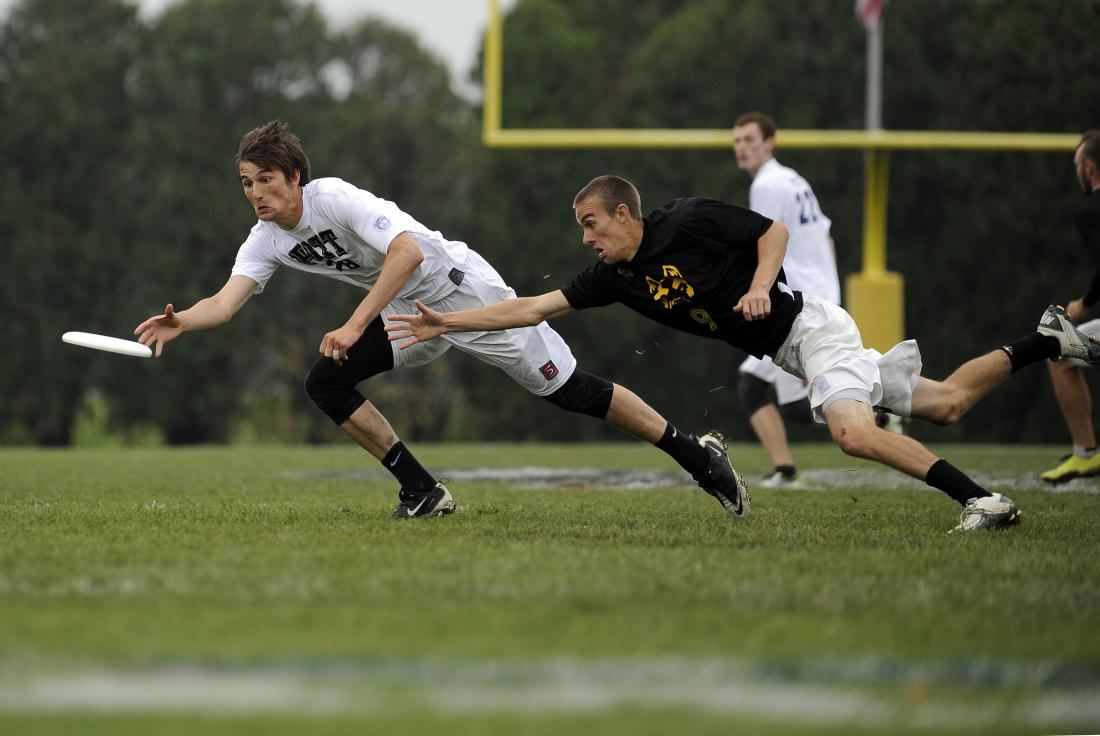
\includegraphics[width=130mm]{./images/ultimate-frisbee.jpg}
\caption{Fotografie z amerického časopisu TIME ze zápasu mezi univerzitními týmy z Pittsburgu a Floridy \cite{ultimate-time}.\label{overflow}}
\end{figure}


\subsection{Spirit of the Game}

\indent

Už od počátku je Ultimate Frisbee založeno na sportovním duchu, který klade odpovědnost
za fair play na samotné hráče. Předpokládá se vysoce soutěživá hra, ne však za cenu ztráty
vzájemné ohleduplnosti a vytracení radosti ze hry. Všechny přetupky na hřišti i mimo něj jsou
řešeny samotnými hráči. Jako jediná sportovní hra se tak obejde bez rozhodčích, a to i
na nejvyšších soutěžích, kterými jsou mistrovství Evropy a světa.

\medskip

Hraní fairplay je otázka cti. Na každém turnaji je vyhlašována cena Spirit of the Game,
která je cenou pro ty, kteří se chovali nejčestněji. Po každém zápase se týmy navzájem ohodnotí
v podobě číselného hodnocení a cenu pak získá tým s nejvyšším průměrem. Cena Spirit of the Game
je ceněna obdobně jako 1. místo.

\subsection{Ultimate v České republice}

\indent

V České republice zastřešuje sporty s létajícím talířem již od roku 1991\cite{cald-historie} Česká asociace
lé\-ta\-jícícho disku (dále jen ``ČALD''). V celé republice eviduje desítky zaregistrovaných
klubů (často zvaných oddílů), které se mezi sebou utkávají v rámci celého roku na akcích zvané turnaje.
Jenom za loňský rok jich bylo na našem území přes třicet \cite{cald-kalendar}.

\medskip

Většina turnajů nebo mistrovství pak trvá zpravidla více dnů, během kterých se odehrají desítky
utkání. A s přibývajícím počtem hráčů a fanoušků vzniká čím dál větší poptávka po online
přenosech a statistikách z těchto akcí.

% TODO: Bude potreba doplnit, protoze se jedna o dulezity pojem, ktery bude pak zpracovan.

%\subsection{Jak probíhá typický turnaj - IDEA - nedokonceno}

%\indent

%Několik dní před turnajem se zveřejní rozpis, zpravidla v podobě dokumentu na Google Drive apod.
%Ten je pak během turnajem editovaný a slouží jako jediný zdroj výsledků, který ... 

%Nejdůležitejším údajem jsou výsledky z jednotlivých zápasů. Ty jsou nejčastěji zapisovány
%na papír, který je vystaven na viditelném místě, aby si jej mohlo prohlédnout co nejvíce lidí.

%\medskip

%Částečně tyto procesy nahrazuje mobilní aplikace Catcher, ke které se ještě dostaneme.

% Vsechno se doposud pise na papir a je to proste cely na prd.
% TODO: Kdo vsechno, kolik lidi, na turnaji pobyva. Kolik probiha zapasu, treba i paralelne, kdo se o nej stara (navrh ma mobilni app). Co vsechno se da vycist z vysledku.

\section{Aplikační rozhraní}

\indent

Častěji se označuje zkratkou API\footnote{Application Programming Interface}.
V informatice se tímto pojmem označuje sbírka procedur, funkcí, tříd
nebo protokolů nějaké knihovny, jež mohou ostatní programátoři používat.
Jde v podstatě o abstrakci, která popisuje rozhraní pro interakci s řadou programových celků,
které programátor využívá namísto toho, aby je sám programoval.
Určuje, jak budou knihovní funkce volány ze zdrojového kódu. API může mít následující vlastnosti.

\begin{itemize}
  % TODO: IDEA: Moznost popsat rozdeleni obecne a konkretni
  \item \textbf{Jazykově závislé API} - Lze volat pouze v daném programovacím jazyce, pomocí základních prvků jazyka.
  \item \textbf{Jazykově nezávislé API} - Jeho použití je možné ve více programovacích jazycích, což je žádoucí vlastnost
    služeb orientovaných na API, které nejsou vázány na určitý systém nebo proces.
    Tato služba pak může být poskytnuta jako webová služba.
\end{itemize}

\section{Protokol HTTP}

\indent

% TODO: Zde bych mel uvest zdroj na cizi diplomku.

Protokol HTTP je základním transportním protokolem na síti internet.
Jde o protokol typu požadavek-odpověď (request-response). Se serverem naváže klient spojení,
odešle mu požadavek a následně obdrží odpověď. Spojení je pak ukončeno.
Požadavek představuje textový dokument, ve kterém dochází ke specifikování paramatru dotazu.
Konkrétní požadavek můžeme vidět na následující ukázce.

\begin{figure}[ht!]
\centering
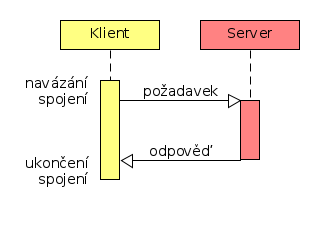
\includegraphics[width=70mm]{./images/http-komunikace.png}
\caption{Sekvenční diagram HTTP komunikace.\label{overflow}}
% TODO: ocitatovat \cite{}
\end{figure}

\begingroup
\fontsize{9.5pt}{11pt}\selectfont
\begin{verbatim}
GET /api/player/1 HTTP/1.1
Host: catcher.zlutazimnice.cz
\end{verbatim}
\endgroup

Na prvním řádku se nachází název HTTP metody (HTTP obsahuje řadu metod, které mají různý význam, více v tabulce ~\ref{tab:http_metody}),
identifikace požadovaného zdroje a verze protokolu. Na následujicích řádcích najdeme tzv. \uv{hlavičky}
(ve formátu \textit{klíč: hodnota}), které specifikují parametry spojení. Jestliže chceme zaslat společně s požadavkem
nějaká data k dalšímu zpracování, umístí se až za hlavičky a jeden prázdný řádek.

\medskip

% TODO: uvest zdroj!!
% TODO: nesouvisi s predchozim: mel bych mozna trochu popsat, co to zdroj je

Odpověď serveru je opět textový dokument, ve kterém se nachází verze protokolu a stavový kód,
který reprezentuje výsledek požadavku. Server může vrátit stavový kód z celkem pěti kategorií,
jejich popis je uveden v tabulce ~\ref{tab:http_kody}. Za stavovým kódem je ještě krátký textový popisek. Na následujících
řádcích jsou hlavičky a výsledek požadavku, který je oddělen opět prázdným řádkem jako v požadavku.
Následující ukázka zobrazuje typickou odpověď z Catchera. 

\begingroup
\fontsize{9.5pt}{11pt}\selectfont
\begin{verbatim}
HTTP/1.1 200 OK
Server: nginx/1.6.3
Date: Mon, 02 May 2016 19:18:18 GMT
Content-Type: application/json; charset=utf-8
Content-Length: 140
Connection: keep-alive
access-control-allow-origin: *
access-control-allow-headers: Content-Type,Authorization,X-Name
access-control-allow-methods: PUT,POST,DELETE,GET

{
  "ranking": null,
  "clubId": 11,
  "firstname": "Pavel",
  "caldId": 976,
  "lastname": "Matoušek",
  "number": 11,
  "nickname": "Maty",
  "id": 1
}
\end{verbatim}
\endgroup

\begin{table}[]
\centering
\begin{tabular}{lp{9.5cm}}
\textbf{Metoda} & \textbf{Význam}\\
\midrule
GET & Základní metoda, jejíž účel je získat požadovaný zdroj. Neměla by mít žádné postraní efekty, jako tvorba nebo mazaní zdrojů.\\
\midrule
POST & Metoda pro odesílání dat ke zpracování (data jsou vložena do těla požadavku). Tato metoda může být použita pro tvorbu nebo úpravu zdrojů.\\
\midrule
DELETE & Metoda určená k mazání zdrojů.\\
\midrule
PUT & Podobně jako POST slouží k odeslání dat ke zpracování.\\
\midrule
\end{tabular}
\caption{Přehled vybraných metod HTTP protokolu v~kontextu této práce \cite{http_metody}.}
\label{tab:http_metody}
\end{table}

\begin{table}[]
\centering
\begin{tabular}{lp{9cm}}
\textbf{Skupina kódů} & \textbf{Význam}\\ \midrule
1xx & Informační kódy.\\ \midrule
2xx & Kódy označující úspěšné vykonání požadavku.\\ \midrule
3xx & Přesměrování - tyto kódy označují odpověď, která obsahuje adresu, na které se nachází požadovaný zdroj.\\ \midrule
4xx & Chybové kódy označující problém při zpracování, způsobený klientem (odeslání nesprávných dat). Před opakováním požadavku je nutné opravit vstupní data.\\ \midrule
5xx & Chybové kódy onzačující problém při zpracování, který vznikl na straně serveru. Požadavek je možné opakovat.\\ \midrule
\end{tabular}
\caption{Kategorie návratových kódů HTTP protokolu [Zdroj: DP VSE].}
% \cite{http_metody}
\label{tab:http_kody}
\end{table}

% TODO: uvest zdroj cizi diplomku

% TODO: Presunout do uvodu.
\section{Webová služba}

\indent

Webová služba je zapouzdřená funkcionalita nějaké aplikace, kterou využívají další aplikace.
Mluvíme tedy o strojové interakci, nevhodné například pro prohlížení ve webovém prohlížeči.
S veřejně vystavenou webovou službou komunikují ostatní aplikace pomocí definovaného rozhraní.
Pro realizaci API se dnes nejčastěji využívají dva protokoly - \textbf{SOAP} a \textbf{REST}.
Tyto protokoly jsou přepravené pomocí již zavedených protokolů (hlavně pomocí HTTP).